\section{Focus group}
The 25th of February 2018, we arranged a focus group at a kitchen in Alrek student home. The participants were:
\textcolor{purple}{TODO Yngve: Flytt navn over i aknowledgements}
\begin{itemize}
	\item 6th year medical doctor student Fredrik Hoel.
	\item 6th year medical doctor student August Hoel.
	\item Master degree student in computer science Mohnd Skr.
	\item Master degree student in computer science Ben-Richard Ebbesvik.
\end{itemize}

As the project was in a very early stage, the purpose of the meeting was exploring how do medical students use CPGs in their training. How the CPGs are used today. How the students work in their practice periods at the hospital. What format are the CPGs in now. What challenges limits the use of CPGs among health workers and medical students at the point of care.

By using a an unstructured interview form, we managed to collect broad and general information, as well as going into detail on interesting topics. As the focus group was small, the contestants could discuss between themselves, highlighting consensus and conflicts \parencite{Preece2015}. A very free and exploitative approach was very successful, as the master degree students in computer science had a very limited knowledge of the medical domain, compared to the medical students. The discussion was documented using an audio recorder.

Topics explored:
\begin{itemize}
	\item The students are learning new medical routines by studying typical cases. Drilling the routines.
	\item Red and yellow flags, which are alarm systems they need to be aware of. A red flag is when the patient's condition is quite critical. What triggers the flags and how to act upon them is something the clinicians need to know by heart, as time is critical and the action needed might be advanced like surgery. No time to use the guidelines. Orange, yellow and green are further degrees of how urgent the clinician's intervention is.  Orange is less urgent than red, but more urgent than yellow. Green is the least urgent one.
	\item Clinicians and medical students use a collection of short guidelines in a pocket book format for references. The guidelines are written mostly in text format and sometimes takes use of tables for presentation.
	\item Mobile devices can't be used at the point of care because of condemnation risks. There are also techniques of consultant with a patient. A mobile device will get in the way for important non-verbal communication.
	\item For departments they need access to specific cases where there isn't much written material. They need access to scientific articles.
	\item They brought up the case where doctors in developing countries have so many patients, and the time to each patient is very limited. To be able to look up information in the guidelines, they need to have a format which makes it very fast to extract that kind of information. Flow-charts is more suitable for developing countries where acting quickly is more often important than in developed countries where they can have a focus on being more thorough in green flag situations.
	\item In addition to guidelines, hospitals can also have their own protocols. The protocols are for situations where the treatment is more specific for this area or hospital. An example is a patient with a blood clot. The medical personnel in Finnmark will start removing the blood clot immediately, because of the long distance to the nearest hospital. They want to reduce the risk for complications. While in Bergen, they will wait with such a treatment. In developing countries you might have to put into consideration what kind of equipment and staff is available at that specific hospital or health care station. The likelihood of different diseases is different from each geographically position, the patients background or the season in the year. Social and economic status also matters, even in Norway.
	\item Discussion about presentation of learning material in an application. Medical cases are often too obvious, too simple or too complicated in existing applications. Flashcards. Show image of an ECG or a picture of a symptom.
	\item Notifying the student about guidelines would be useful. But only for the most common and dangerous conditions, relevant for the students medical field to avoid unnecessary notifications which will only be ignored.
%	The statistically most common and dangerous conditions first.
%	Then look for signs where you can rule out conditions. Elimineringsmetoden
\item The diagnostic process. The doctor have several conditions in mind, but tries to eliminate the statistically most common and dangerous first. Trying to narrow down the alternatives until the doctor is quite certain about the medical condition of the patient.
	
\end{itemize}


\section{Workshop}
The 22nd of February 2019 we had a workshop. The purpose of the workshop was to
\begin{itemize}
	\item Identify components in the treatment plan of asthma patients.
	\item Identify difficulty levels, and how the questions will be more detailed for every difficulty level.
	\item Make a map of the learning content. Where the content is categorized in components and difficulty levels.  Identify paths the student can take through the learning content.f 
\end{itemize}

\textcolor{purple}{TODO: Move names over in aknowledgements}
The antecedences for the meeting was 
\begin{itemize}
	\item Professor in computer science Yngve Lamo. Background in model driven engineering and health informatics.
	\item Assistant professor in computer science Svein Ivar Lillehaug. Background as a researcher in health informatics.
	\item Postdoctoral fellow Fazle Rabbi. Background in model driven engineering.
	\item Medical doctor and PhD student in health informatics Job Nyangena.
	\item PhD research fellow in interaction design Rosaline Barendregt. Has written a master thesis in gamification.
	\item PhD candidate in computer science and health informatics Suresh Kumar Mukhiya.
	\item Master degree student in computer science Ben-Richard Ebbesvik.	
\end{itemize}

\begin{figure}[h!]
	\caption {Anticlockwise from front left: Yngve Lamo, Rosaline Barendregt, Suresh Kumar Mukhiya, Svein Ivar Lillehaug, Fazle Rabbi and Job Nyangena}
	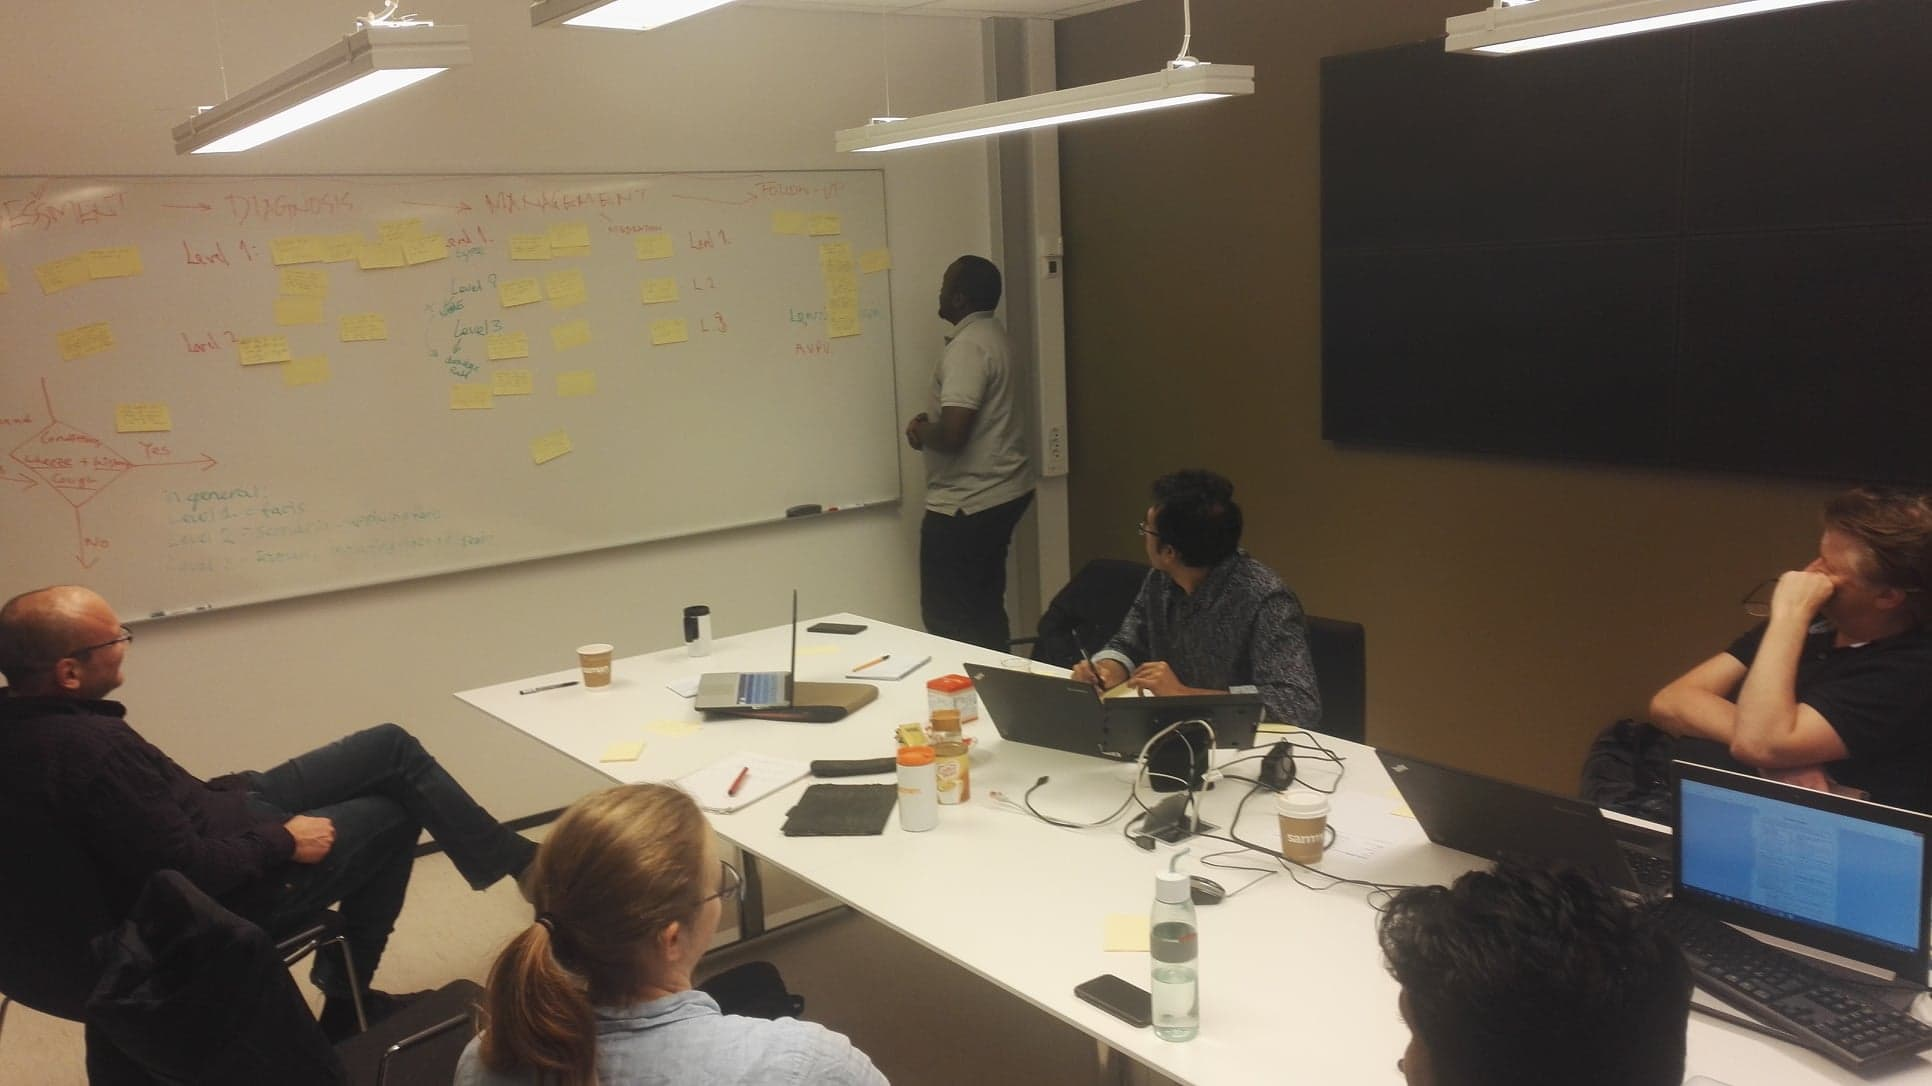
\includegraphics[scale=0.25]{workshop220219}
\end{figure}

The meeting started with Ben-Richard informing the status of the project by doing a cognitive walk-through and a demonstration of the application. 

Yngve presented ideas for further development of the application. The important thing, was the concept of splitting up the questions in themes which relates to components in the treatment plan. Job helped identify these themes as assessment, diagnosis, management and treatment. Further we identified what type of questions we wanted to ask, and how they fits into different difficulty levels, based on the details of the questions. We ask factual questions for level 1. We use scenarios in level 2, where we apply facts and the detail level is categories. I.e. what class of medication should be administered to the patient. In level 3 we continue with scenarios, but here we ask for much more details, like the dosage of a medication or how often it should be administered.

\textcolor{purple}{TODO Yngve: Eksempel}

When playing level 1 the student should get questions from all themes in level 1. When the student completes level 1, the student should no longer get questions from that theme. This is to avoid boring the user by repeating the questions the student already knows the answer of. He should only get questions from themes he struggles with. I.e. on the first run level 1, the user gets every question in assessment right, but have some mistakes with diagnosis and management. Then on the next run, he only gets questions from level 1 diagnosis and management. This continues until he has reached the passing condition on every theme in level 1. 

We further identified a dependency in the treatment plan. To be able to do a follow-up, the students first needs to know something about assessment, diagnosis and management of the patient. The follow-up is actually an evaluation of the treatment which have been given, based on the suggested diagnosis. The evaluation will tell how the patient responded to the treatment, and the student needs to take actions whether the patient responded or his condition became better or worse. When we have such a dependency, the student needs to complete assessment, diagnosis and management before follow-up gets unlocked. Since follow-up is only relevant in a situation where there has already been set a diagnosis and given a treatment, the follow-up is only part of level 2 and 3, where the questions are given as scenarios.

\textcolor{purple}{TODO Yngve: Vis en graf der follow-up blir låst opp}

To complete a level, all passing conditions at that level in each theme have to be met. When the student qualifies for a new level, he only gets questions from the level he plays. The same concept of only getting questions from the themes at that level you haven't met the passing condition, continues for level 2 and 3. 

We planned to have a visualization of the passing condition in the application. The passing condition will be shown in a chart in the summary section after each game. The passing condition will be marked as a line over every theme for the level the student plays. The students scores for each theme at that level be shown as bars. When a bar reaches the line, a passing condition is met.




\begin{figure}[h!]
	\caption {Assessment and diagnosis are components in the treatment plan. In the learning map they are themes. Under each theme there are difficulty levels. Questions for each level are written on post-it notes.}
	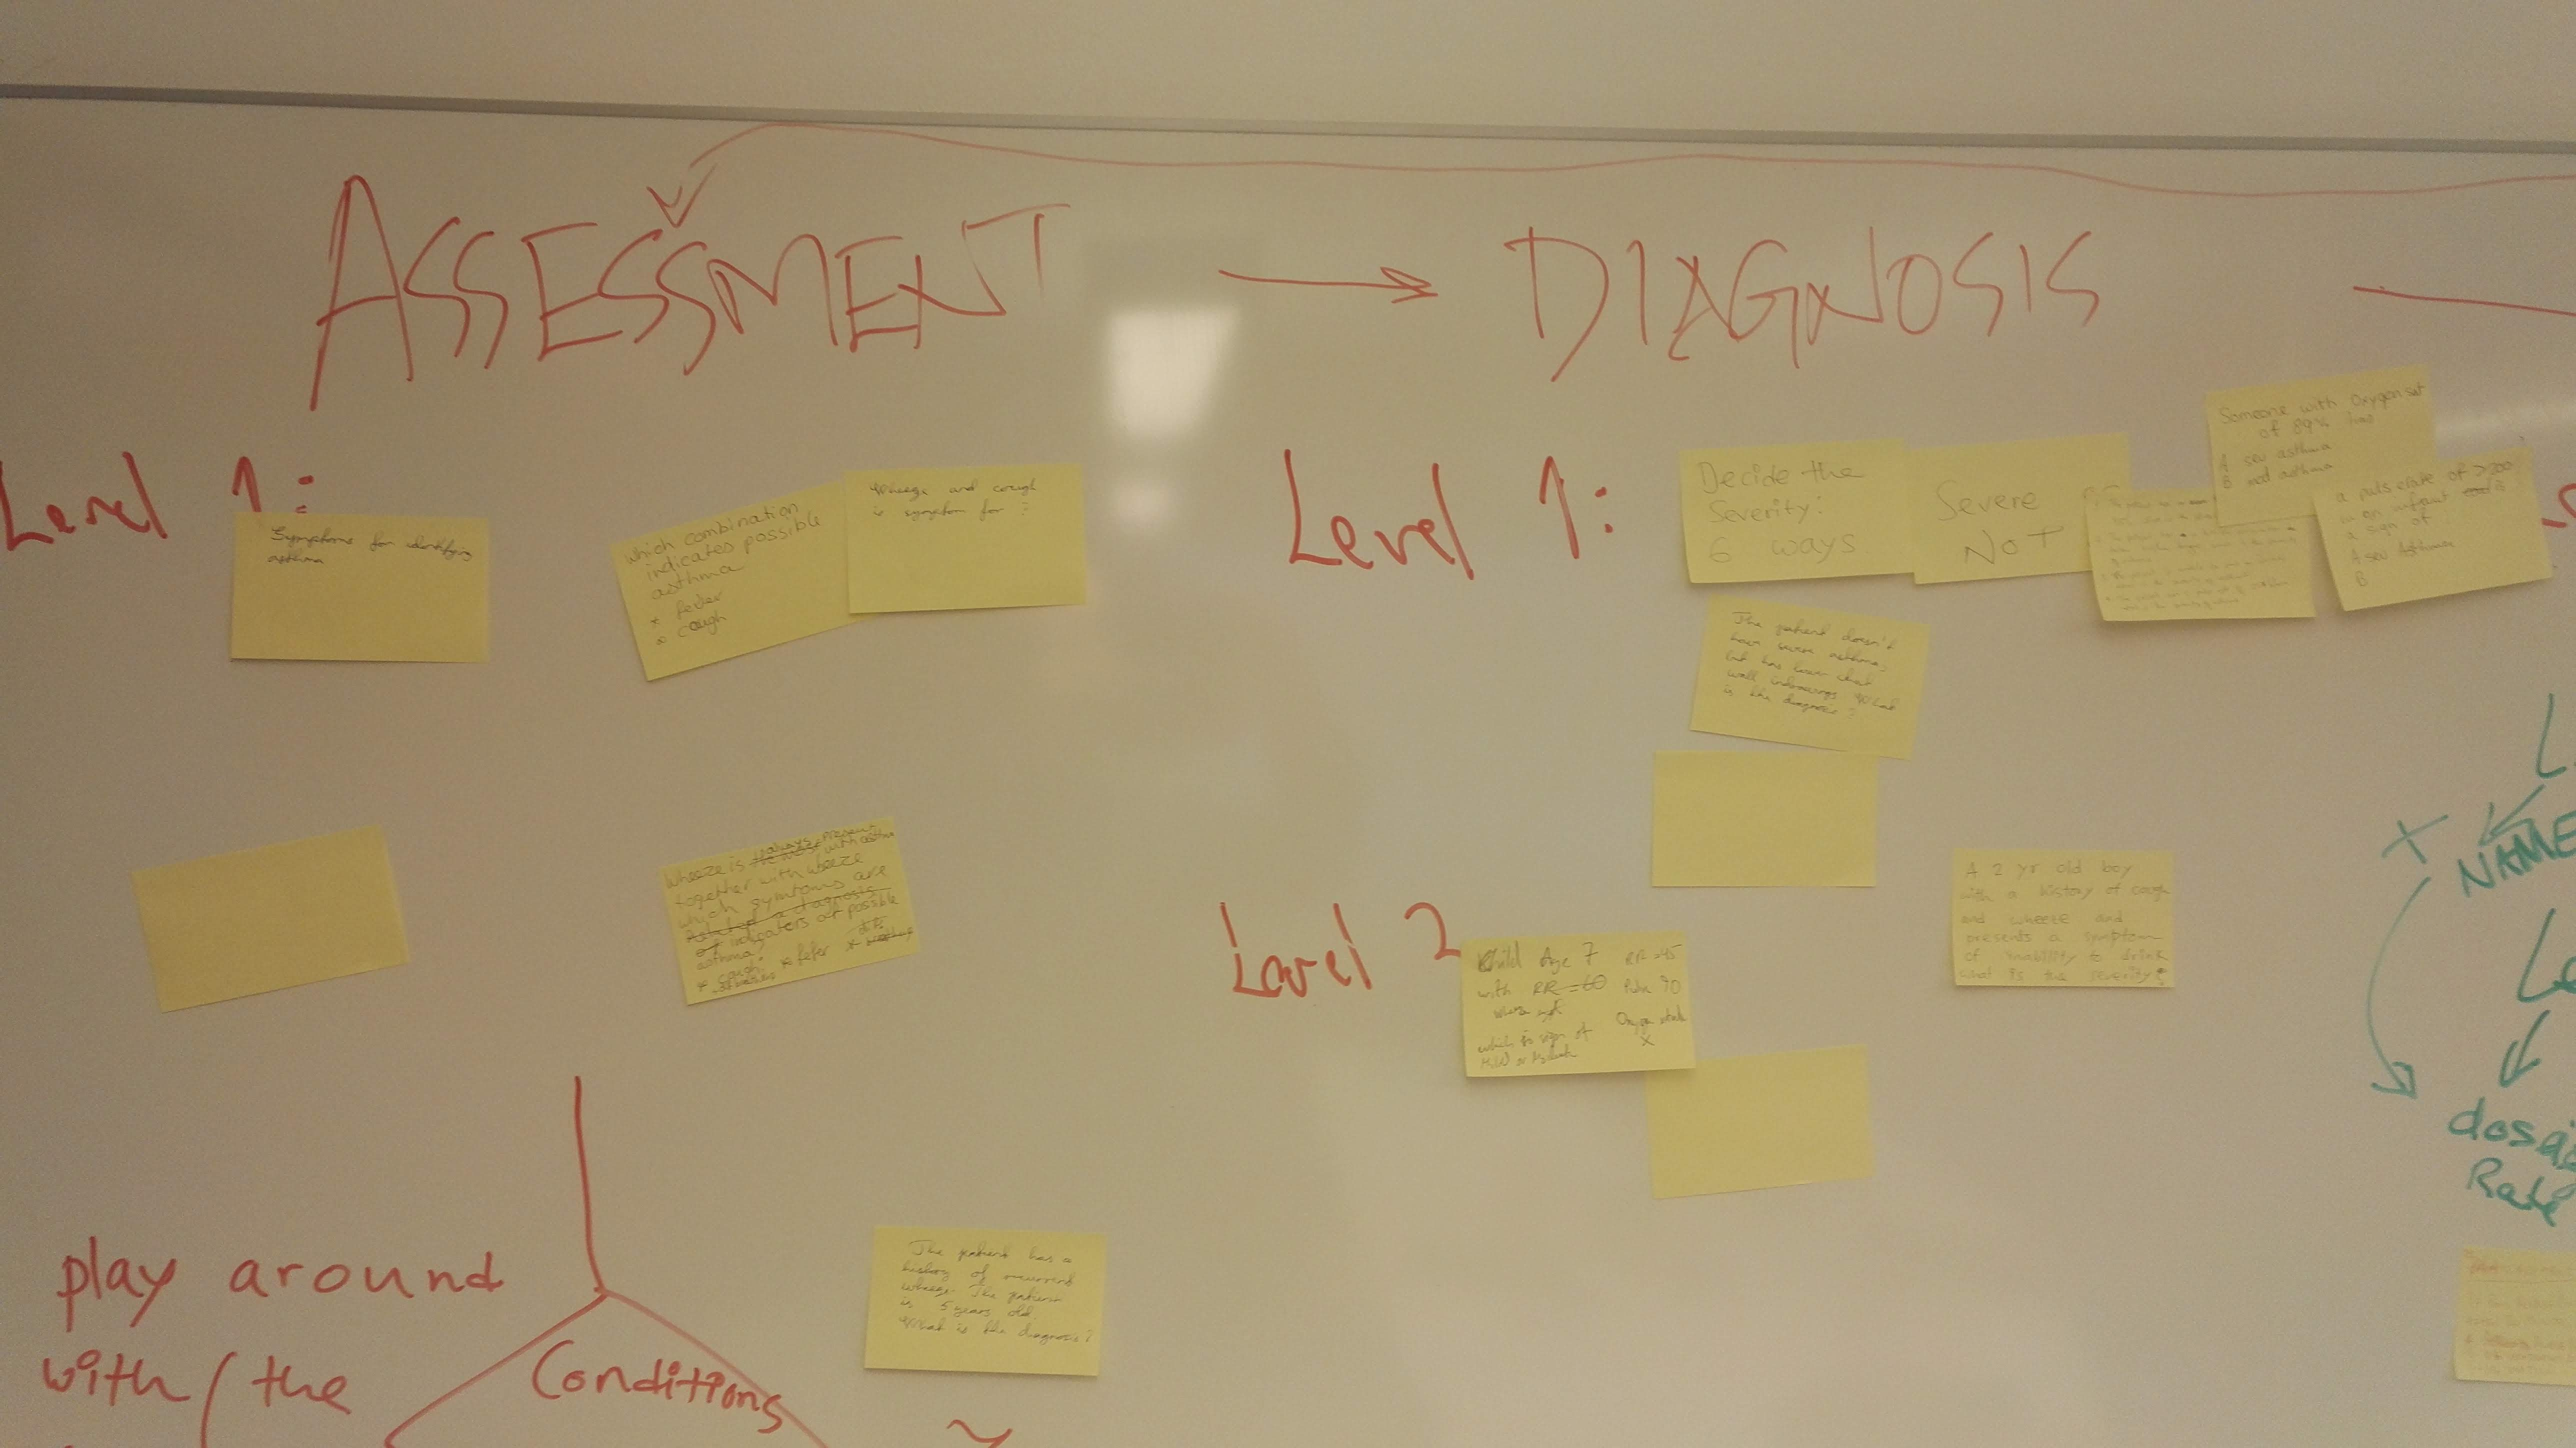
\includegraphics[scale=0.075]{workshop220219-2}
\end{figure}

\begin{figure}[h!]
	\caption {Management and follow-up are components in the treatment plan. In the learning map they are themes. Under each theme there are difficulty levels. Questions for each level are written on post-it notes.}
	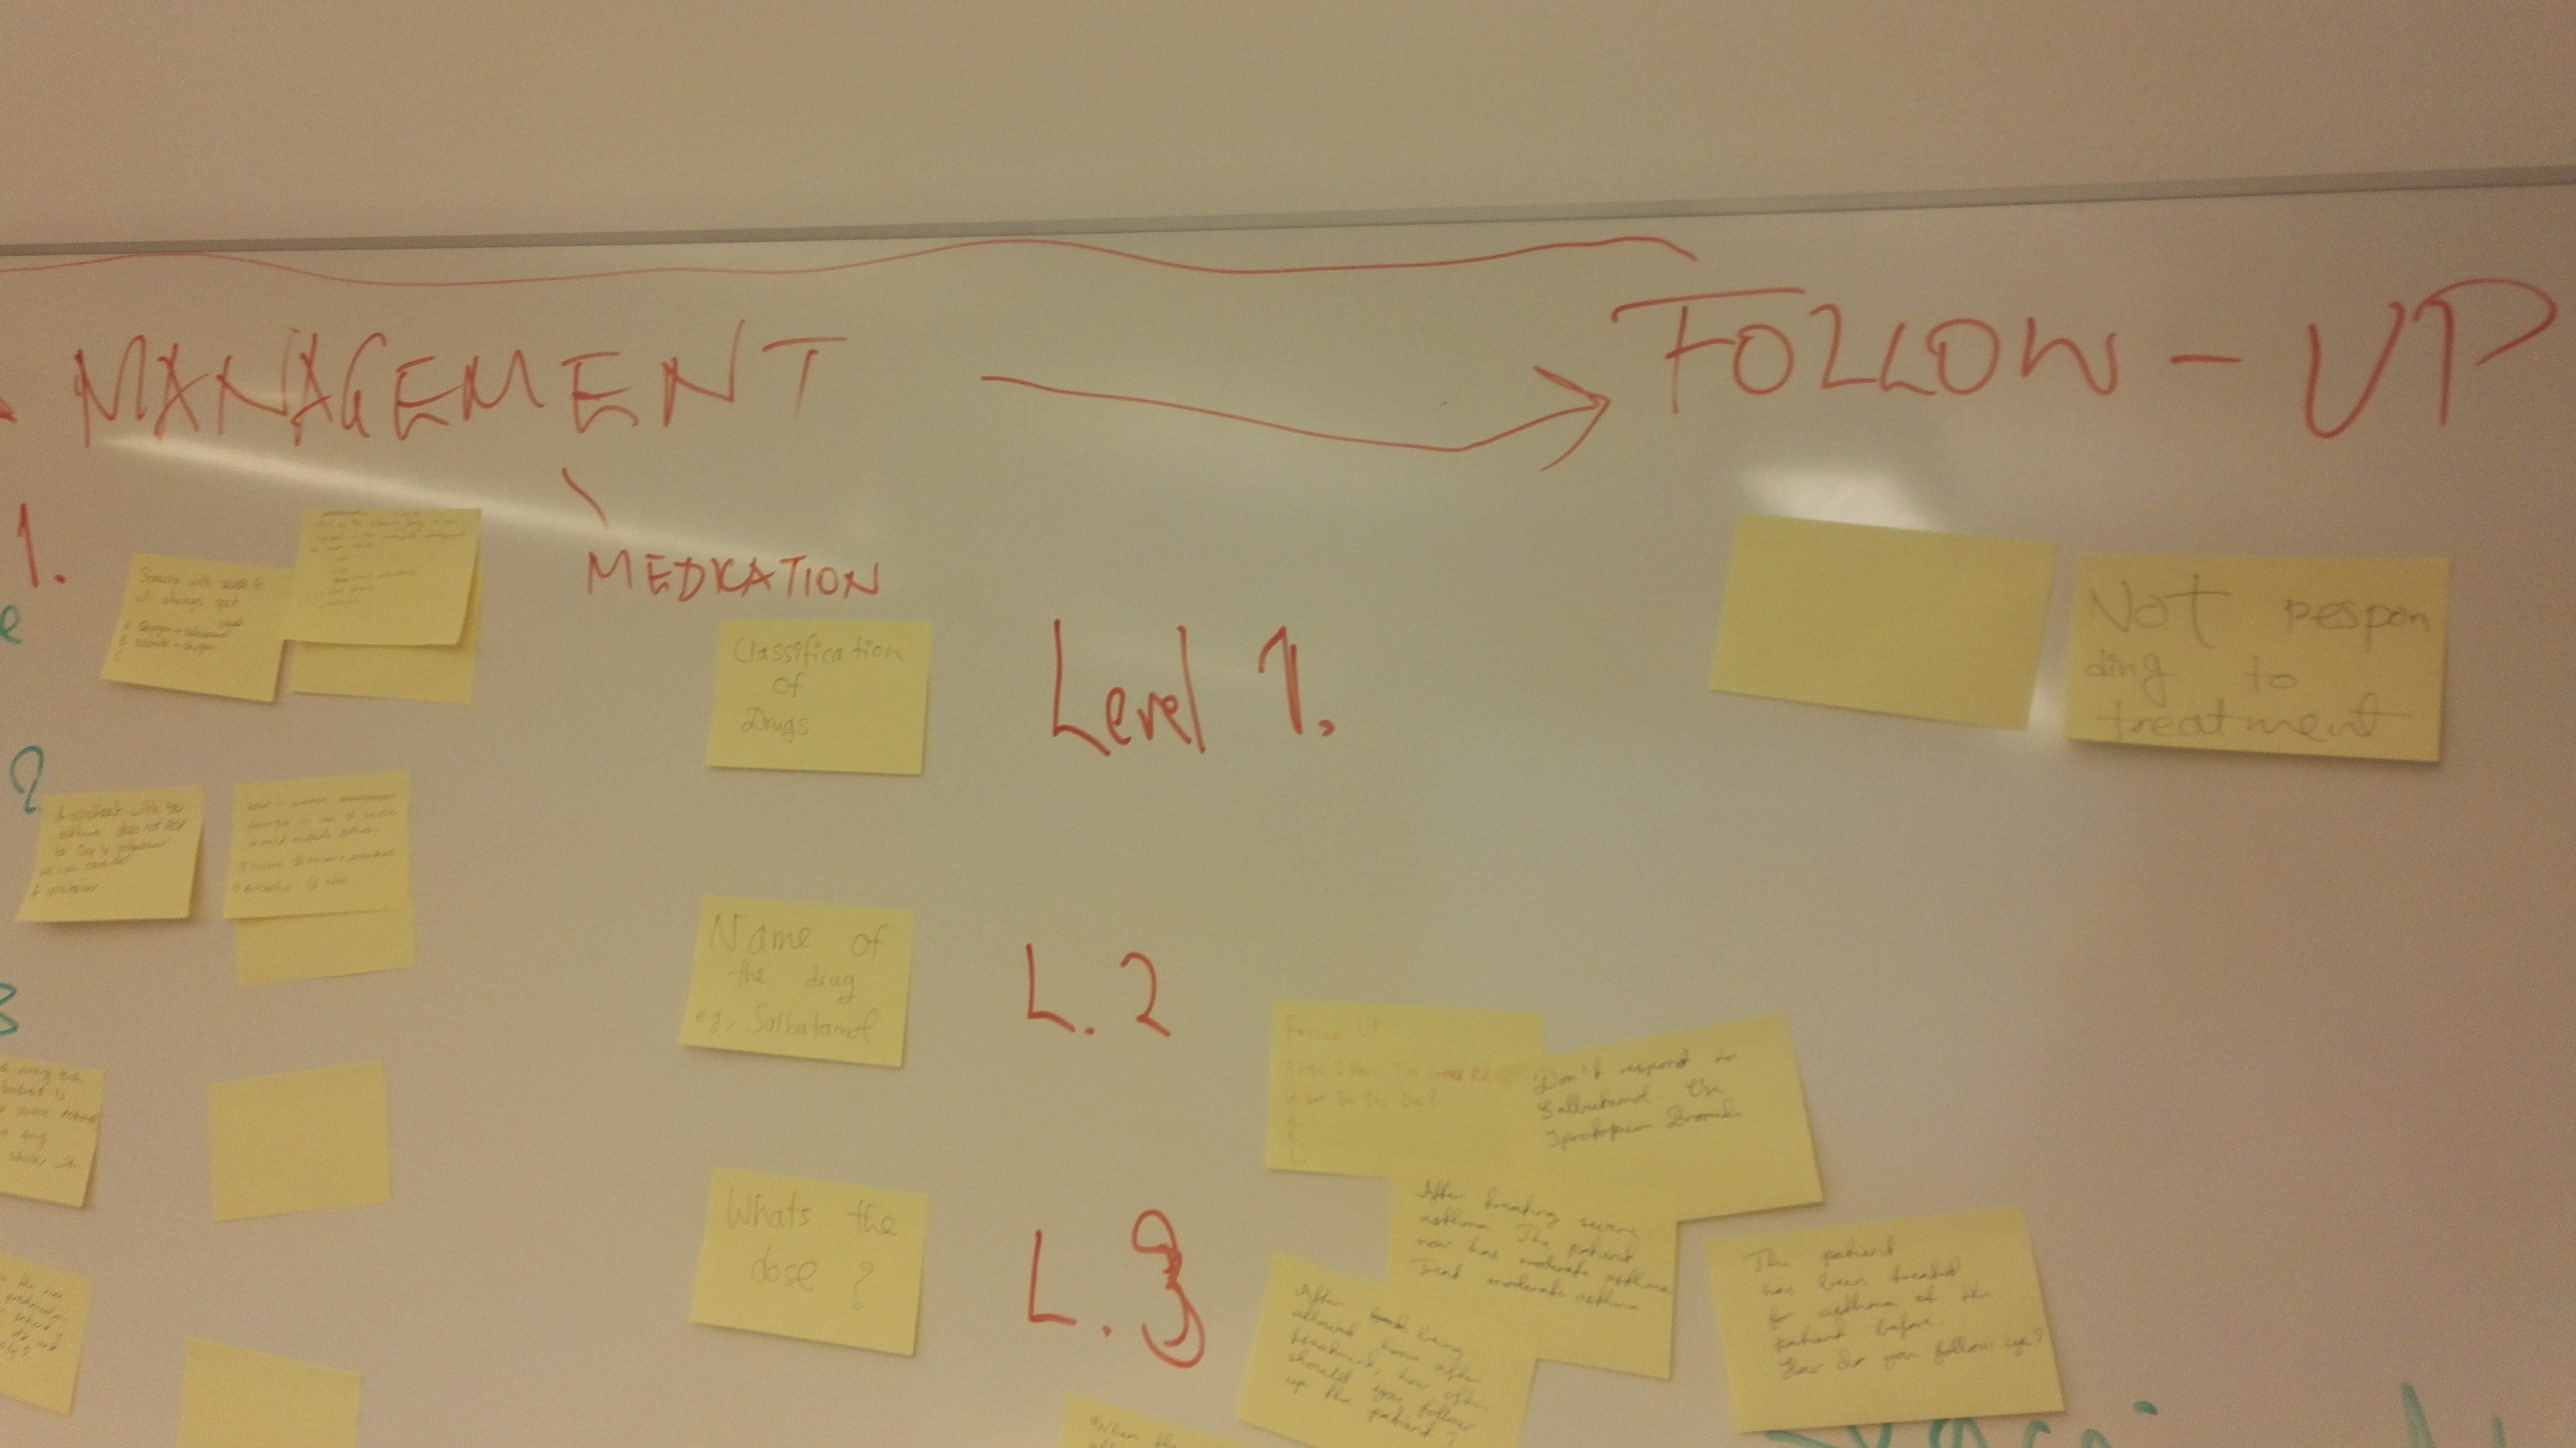
\includegraphics[scale=0.075]{workshop220219-3}
\end{figure}

\begin{figure}[h!]
	\caption {What type of questions the student will get at each level.}
	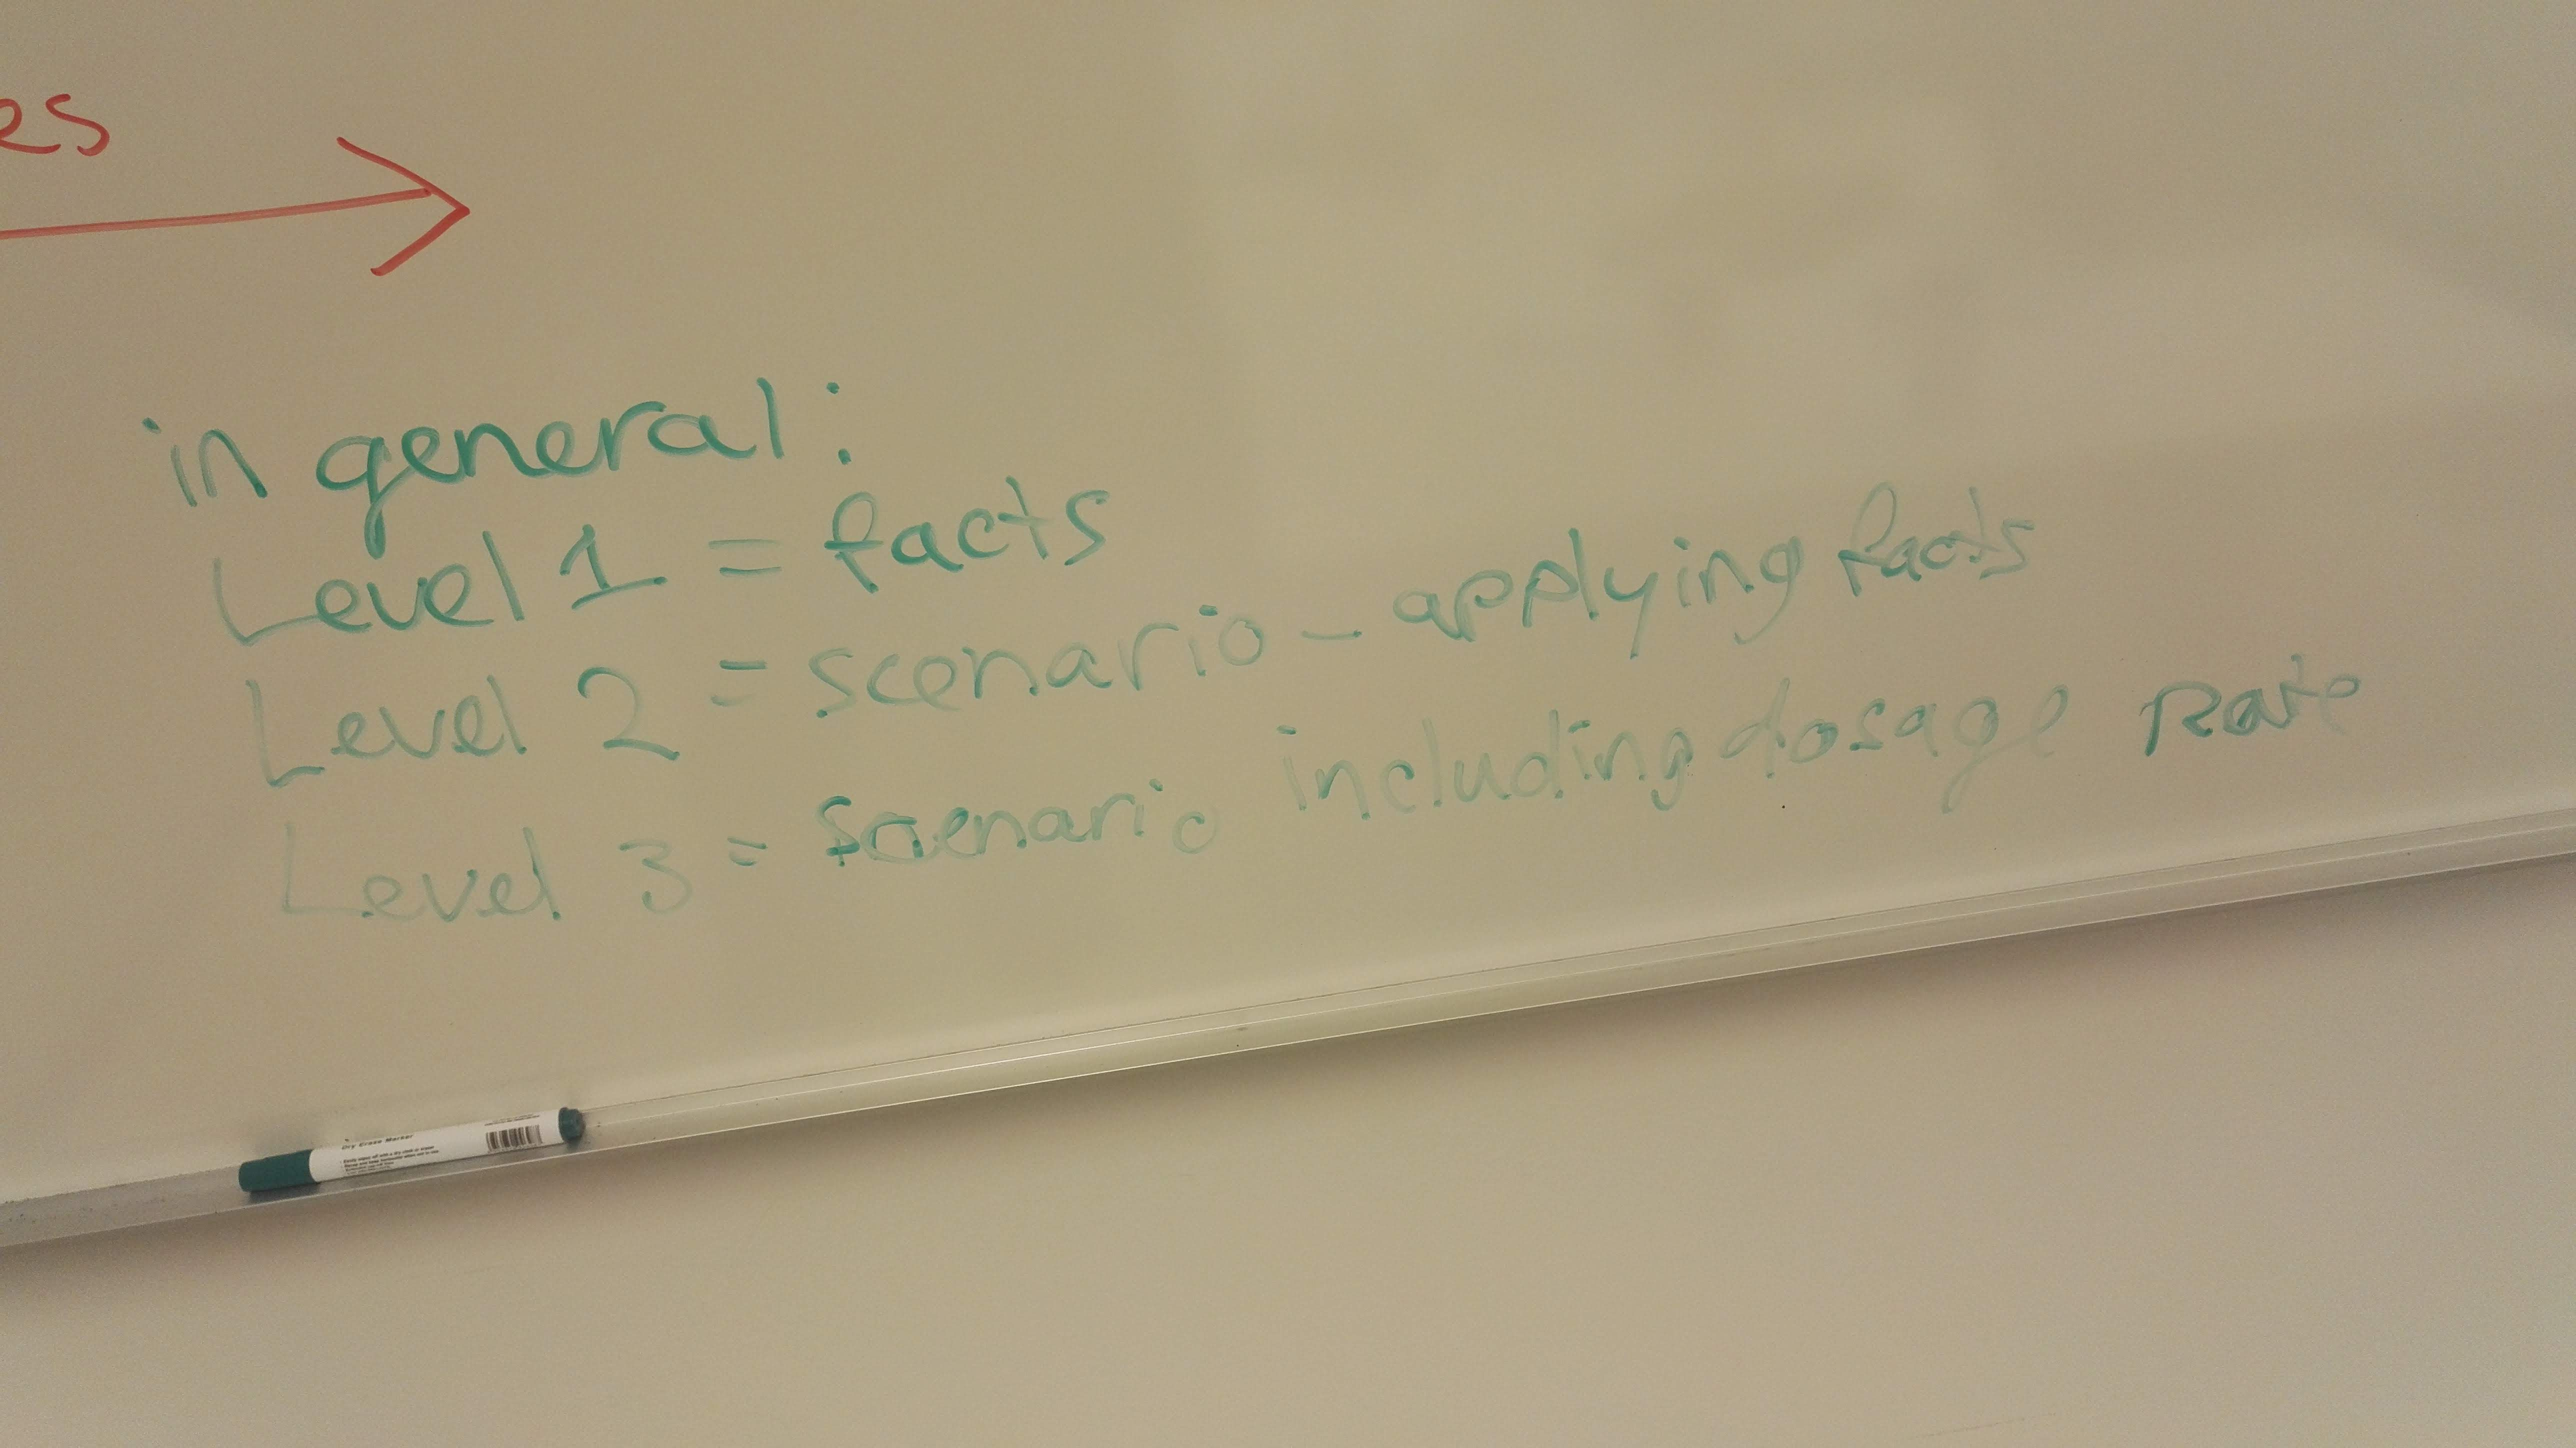
\includegraphics[scale=0.075]{workshop220219-4}
\end{figure}

Job continued the meeting by talking about the guidelines.The paediatric guideline of asthma is called "possible asthma". That is because in an emergency situation asthma is the most dangerous airway condition and can be lethal. If the patient shows signs of asthma, he will be treated for asthma to reduce risks of an unwanted scenario.

We identified users of the application: 
\begin{itemize}
	\item Formal training, where last year medical students are reading for their exams.
	\item Anyone can learn, so it can be used to inform and educate the public.
	\item In countries such as Kenya, where there are a large deficit in doctors and nurses, sometimes nurses has to work as doctors. Or community workers need to take the role as doctor or nurse. The application will help educating nurses and community workers for such scenarios.
\end{itemize}
 
 There was also talked about how the situation in medical training is for the student. When a patient comes to the emergency room with severe asthma, the medical doctors will have all their focus on that particular patient. The medical student will typically not take part in the assessment, diagnosis or the initial treatment of the patient. The medical student will typically only take part in the monitoring, evaluation and follow-up of the patient, when the situation is less critical. The application will give the medical student an alternative way to train in assessment, diagnosis and initial treatment of a made-up patient with severe asthma. 

Job continued the workshop by going through the Kenyan paediatric guideline of possible asthma \parencite{RepublicofKeny2016}. This is the guideline we will base our quiz on. Job answered questions from the group about details of the guideline. It is important to understand the general flow as well as the details to be able to make good questions for the quiz. The guidelines is poorly written in terms of wrong use of sentential operators. These mistakes needed to be clarified.

The rest of the workshop was for the participants brainstorming around the questions which will be used in the quiz. Each participant wrote questions on post-it notes, and placed them at a suiting level and theme on the blackboard. At the end, Job went through the questions and we had a small discussion around the suggested questions. We managed to produce question templates to be used in asthma quiz of the application.

\begin{figure}[h!]
	\caption {Suggestions for questions were written on post-it notes and attached to a difficulty level under a theme on the black board.}
	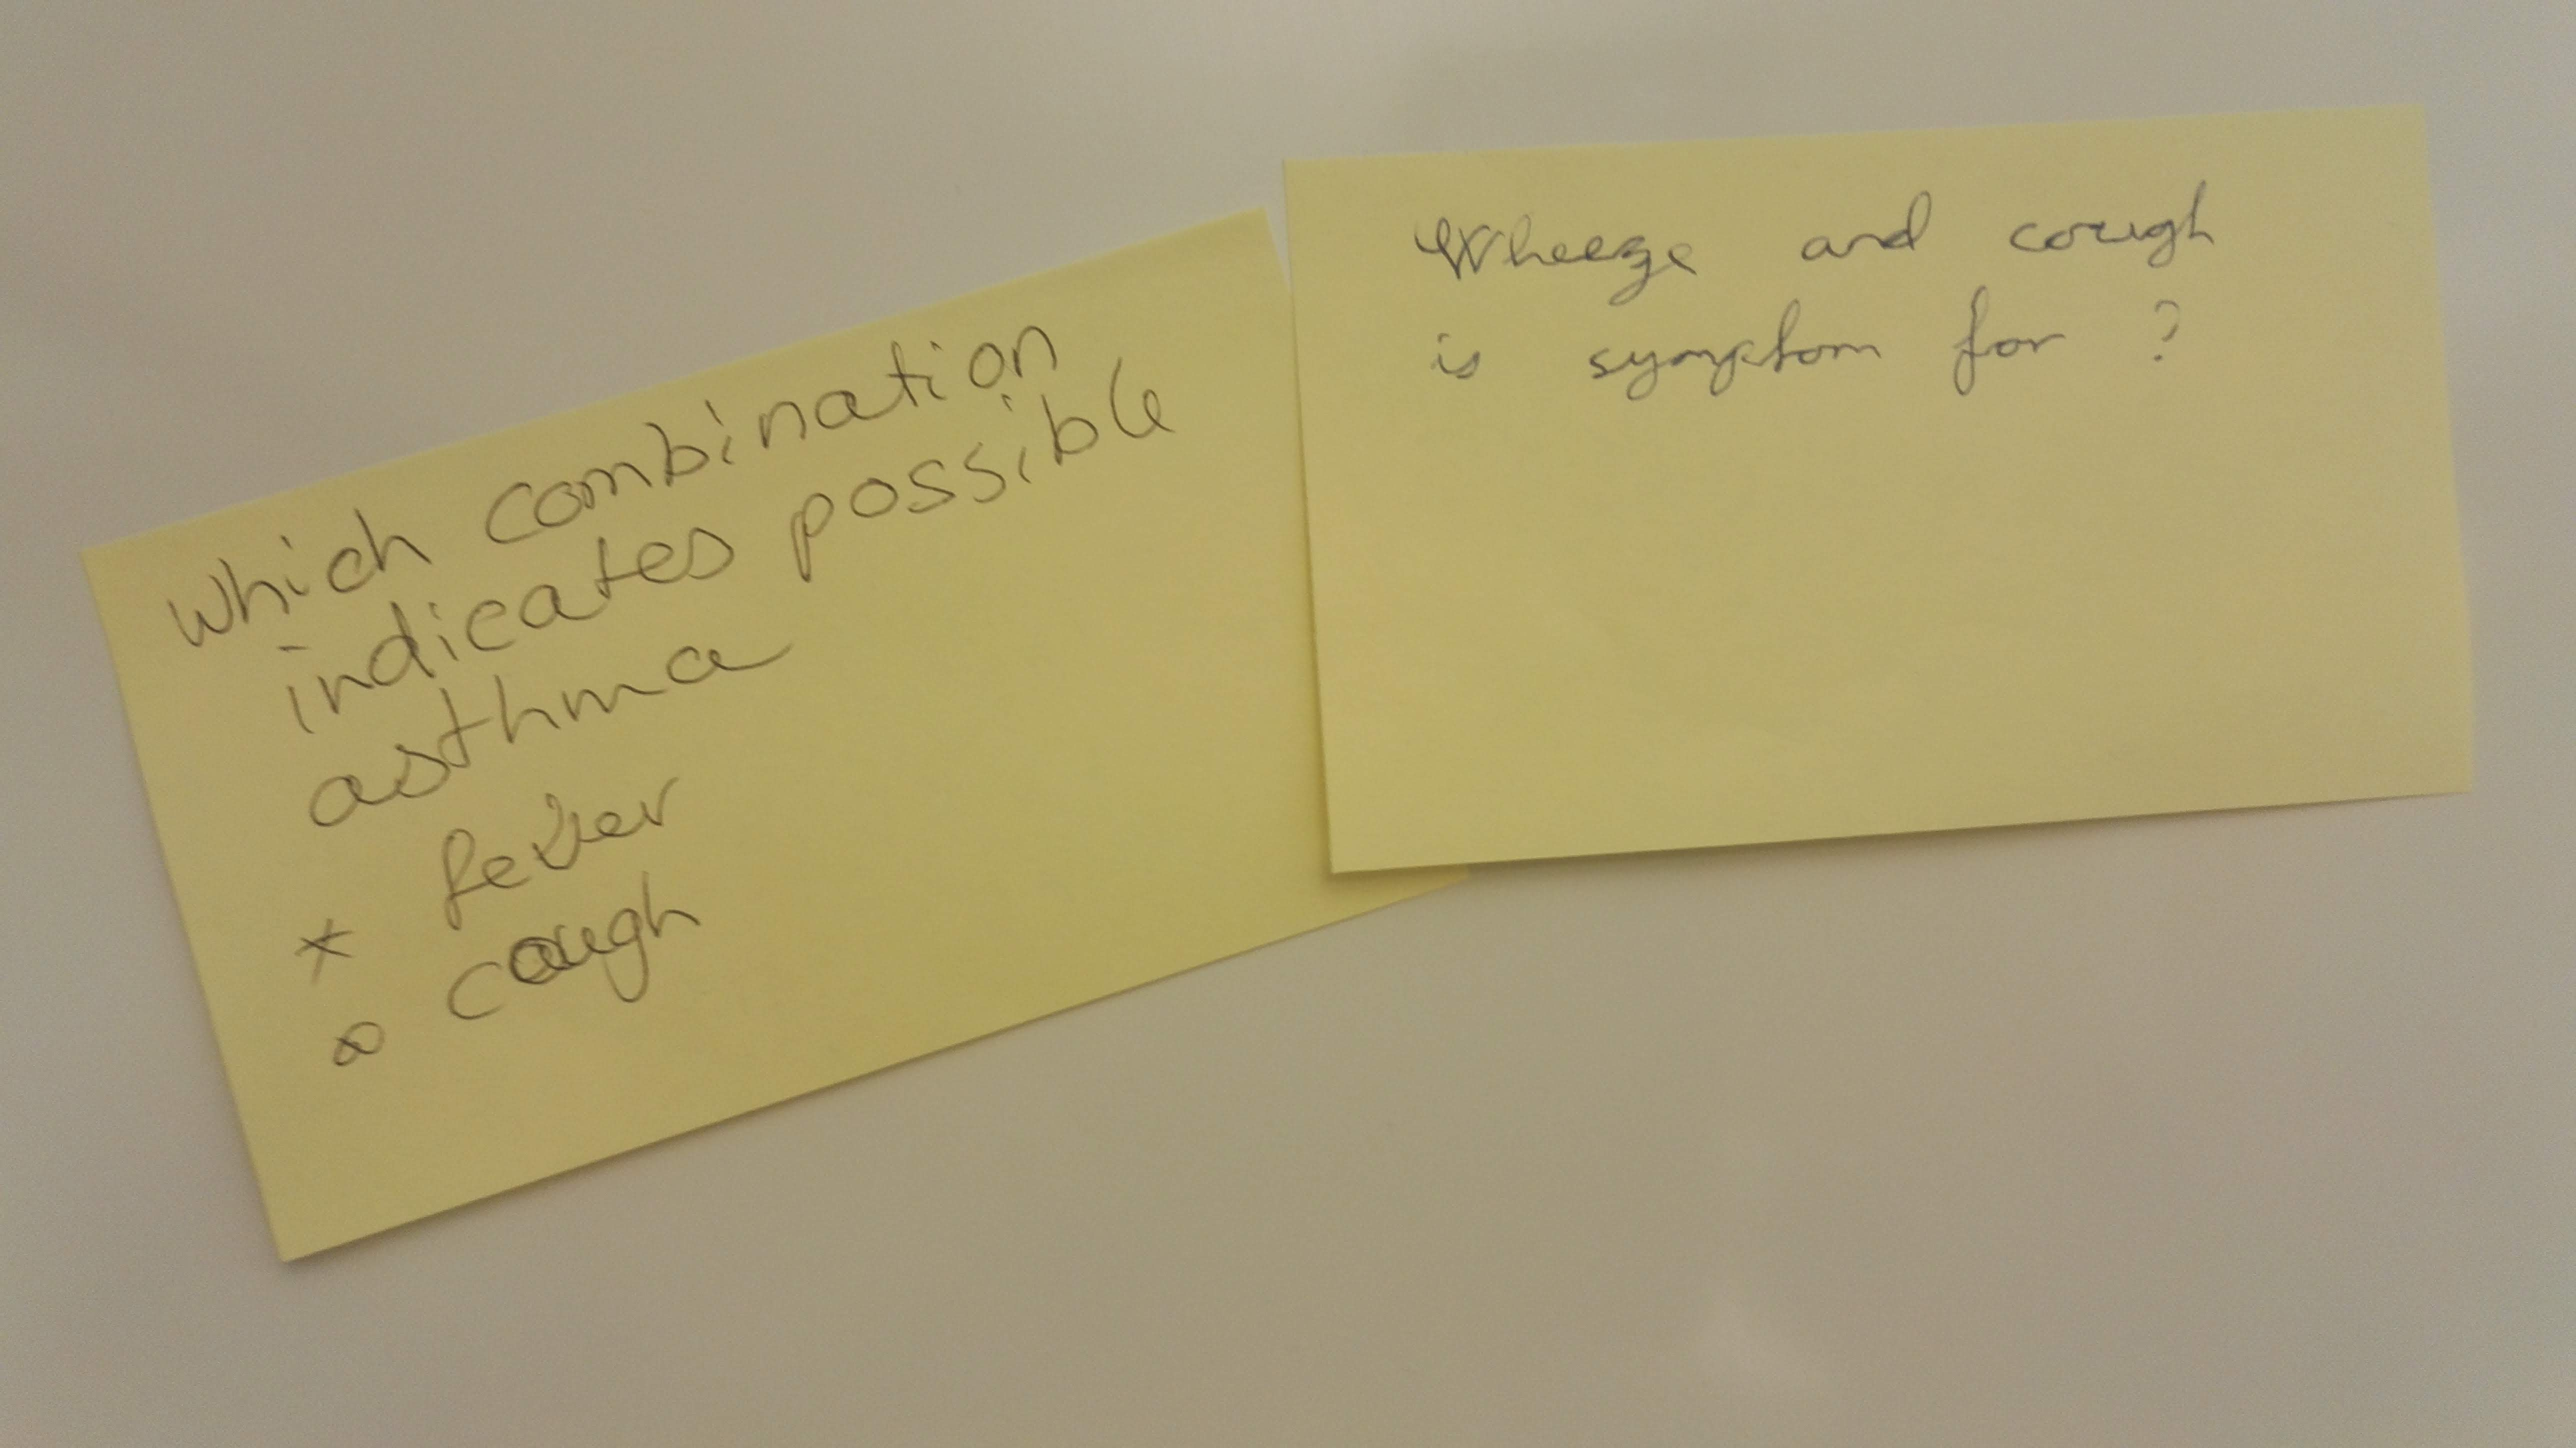
\includegraphics[scale=0.075]{workshop220219-5}
\end{figure}